\documentclass[a4paper]{book}
\usepackage{a4wide}
\usepackage{makeidx}
\usepackage{graphicx}
\usepackage{multicol}
\usepackage{float}
\usepackage{listings}
\usepackage{color}
\usepackage{textcomp}
\usepackage{alltt}
\usepackage{times}
\usepackage{ifpdf}
\ifpdf
\usepackage[pdftex,
            pagebackref=true,
            colorlinks=true,
            linkcolor=blue,
            unicode
           ]{hyperref}
\else
\usepackage[ps2pdf,
            pagebackref=true,
            colorlinks=true,
            linkcolor=blue,
            unicode
           ]{hyperref}
\usepackage{pspicture}
\fi
\usepackage[utf8]{inputenc}
\usepackage{doxygen}
\lstset{language=C++,inputencoding=utf8,basicstyle=\footnotesize,breaklines=true,breakatwhitespace=true,tabsize=8,numbers=left }
\makeindex
\setcounter{tocdepth}{3}
\renewcommand{\footrulewidth}{0.4pt}
\begin{document}
\hypersetup{pageanchor=false}
\begin{titlepage}
\vspace*{7cm}
\begin{center}
{\Large Reference Manual}\\
\vspace*{1cm}
{\large Generated by Doxygen 1.6.1}\\
\vspace*{0.5cm}
{\small Thu Oct 16 22:23:35 2014}\\
\end{center}
\end{titlepage}
\clearemptydoublepage
\pagenumbering{roman}
\tableofcontents
\clearemptydoublepage
\pagenumbering{arabic}
\hypersetup{pageanchor=true}
\chapter{Class Index}
\section{Class Hierarchy}
This inheritance list is sorted roughly, but not completely, alphabetically:\begin{DoxyCompactList}
\item \contentsline{section}{input\_\-format\_\-error}{\pageref{classinput__format__error}}{}
\item \contentsline{section}{invalid\_\-coordinates\_\-error}{\pageref{classinvalid__coordinates__error}}{}
\item \contentsline{section}{invalid\_\-line\_\-error}{\pageref{classinvalid__line__error}}{}
\item \contentsline{section}{invalid\_\-screen\_\-error}{\pageref{classinvalid__screen__error}}{}
\item \contentsline{section}{Screen}{\pageref{classScreen}}{}
\item \contentsline{section}{ScreenElement}{\pageref{classScreenElement}}{}
\begin{DoxyCompactList}
\item \contentsline{section}{Box}{\pageref{classBox}}{}
\begin{DoxyCompactList}
\item \contentsline{section}{TextBox}{\pageref{classTextBox}}{}
\end{DoxyCompactList}
\item \contentsline{section}{Line}{\pageref{classLine}}{}
\item \contentsline{section}{Text}{\pageref{classText}}{}
\begin{DoxyCompactList}
\item \contentsline{section}{TextBox}{\pageref{classTextBox}}{}
\end{DoxyCompactList}
\end{DoxyCompactList}
\end{DoxyCompactList}

\chapter{Class Index}
\section{Class List}
Here are the classes, structs, unions and interfaces with brief descriptions:\begin{DoxyCompactList}
\item\contentsline{section}{\hyperlink{classBox}{Box} }{\pageref{classBox}}{}
\item\contentsline{section}{\hyperlink{classinput__format__error}{input\_\-format\_\-error} (An error which is thrown when the given input does not meet the desired format )}{\pageref{classinput__format__error}}{}
\item\contentsline{section}{\hyperlink{classinvalid__coordinates__error}{invalid\_\-coordinates\_\-error} (An error which is thrown when the given coordinated are out of range )}{\pageref{classinvalid__coordinates__error}}{}
\item\contentsline{section}{\hyperlink{classinvalid__line__error}{invalid\_\-line\_\-error} (An error which is thrown when a line is created that is not vertical or horizontal )}{\pageref{classinvalid__line__error}}{}
\item\contentsline{section}{\hyperlink{classinvalid__screen__error}{invalid\_\-screen\_\-error} (An error which is thrown when the user tried to add objects to the screen before the screen is created )}{\pageref{classinvalid__screen__error}}{}
\item\contentsline{section}{\hyperlink{classLine}{Line} }{\pageref{classLine}}{}
\item\contentsline{section}{\hyperlink{classScreen}{Screen} }{\pageref{classScreen}}{}
\item\contentsline{section}{\hyperlink{classScreenElement}{ScreenElement} }{\pageref{classScreenElement}}{}
\item\contentsline{section}{\hyperlink{classText}{Text} }{\pageref{classText}}{}
\item\contentsline{section}{\hyperlink{classTextBox}{TextBox} }{\pageref{classTextBox}}{}
\end{DoxyCompactList}

\chapter{Class Documentation}
\hypertarget{classBox}{
\section{Box Class Reference}
\label{classBox}\index{Box@{Box}}
}


{\ttfamily \#include $<$Box.h$>$}Inheritance diagram for Box::\begin{figure}[H]
\begin{center}
\leavevmode
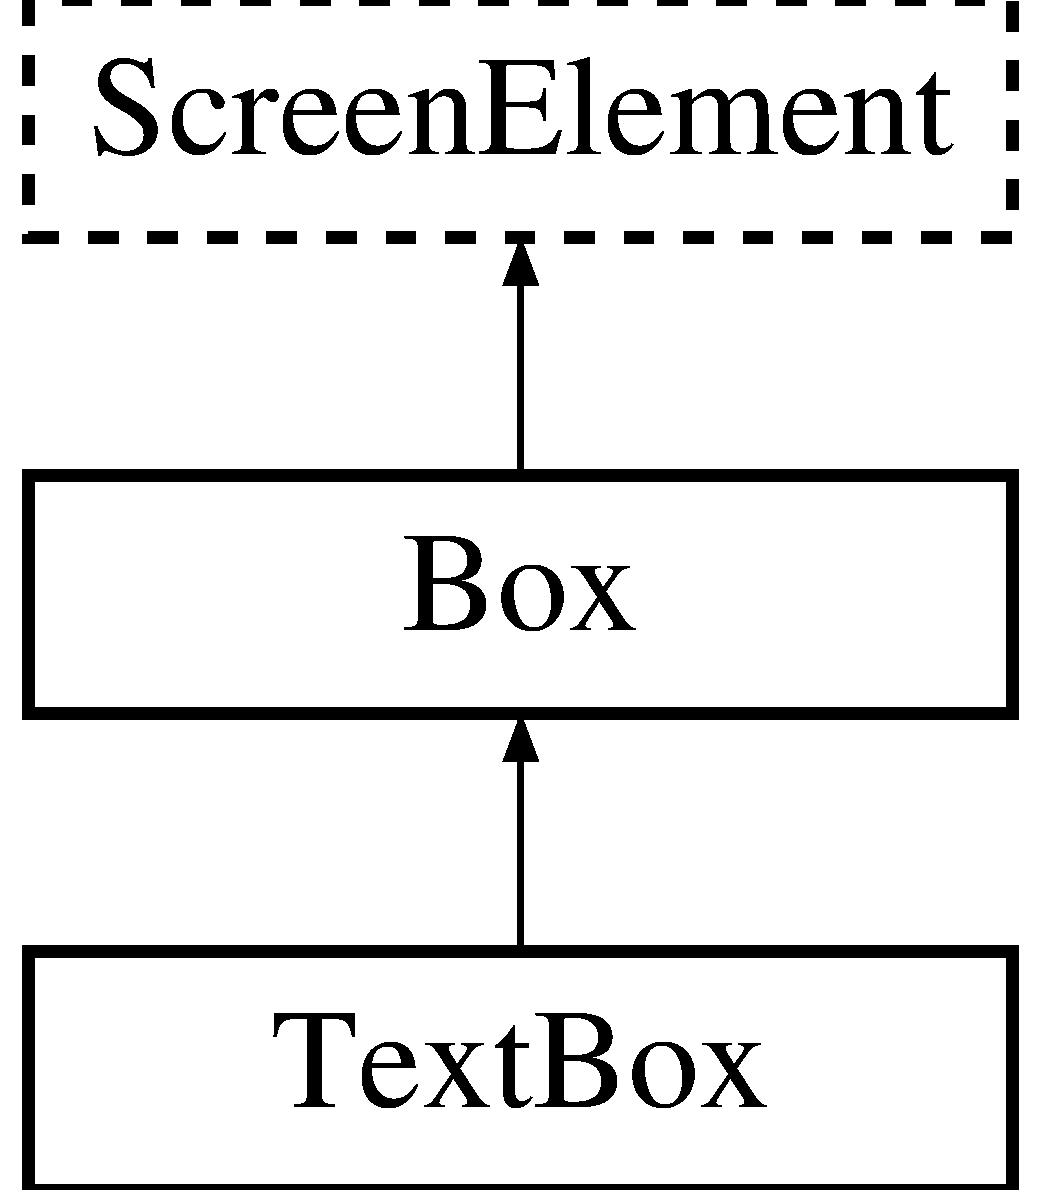
\includegraphics[height=3cm]{classBox}
\end{center}
\end{figure}
\subsection*{Public Member Functions}
\begin{DoxyCompactItemize}
\item 
\hyperlink{classBox_a77fa7ad8be8934cbe9c3bcc86ca33998}{Box} (int ul\_\-row=0, int ul\_\-column=0, int br\_\-row=0, int br\_\-column=0, char ch= ' ')
\item 
virtual void \hyperlink{classBox_a5c6c1c650b13f2978e3b559bb5af15d2}{draw} (\hyperlink{classScreen}{Screen} \&screen)
\begin{DoxyCompactList}\small\item\em draws the \hyperlink{classBox}{Box} on the given \hyperlink{classScreen}{Screen} \item\end{DoxyCompactList}\item 
virtual void \hyperlink{classBox_ac0ea633a10bf980901766b7aaefdb912}{read} (istream \&is)
\end{DoxyCompactItemize}
\subsection*{Protected Member Functions}
\begin{DoxyCompactItemize}
\item 
void \hyperlink{classBox_a5411fa40529560030450d1eee001623d}{constructLines} (int ul\_\-row, int ul\_\-column, int br\_\-row, int br\_\-column, char ch)
\end{DoxyCompactItemize}
\subsection*{Protected Attributes}
\begin{DoxyCompactItemize}
\item 
\hypertarget{classBox_a1b0489e286b8bf52c2f38c7042a5e617}{
\hyperlink{classLine}{Line} \hyperlink{classBox_a1b0489e286b8bf52c2f38c7042a5e617}{m\_\-line} \mbox{[}4\mbox{]}}
\label{classBox_a1b0489e286b8bf52c2f38c7042a5e617}

\begin{DoxyCompactList}\small\item\em the four Lines that make up a box \item\end{DoxyCompactList}\end{DoxyCompactItemize}


\subsection{Detailed Description}
The \hyperlink{classBox}{Box} class is an abstraction of a retangular box that can be drawn on a \hyperlink{classScreen}{Screen}. It is specified internally by two corners-\/-\/-\/upper left and bottom right, as well as a character to draw the box with. It provides functions to draw itself on a \hyperlink{classScreen}{Screen} as well as reading a description of itself from an input stream. 

\subsection{Constructor \& Destructor Documentation}
\hypertarget{classBox_a77fa7ad8be8934cbe9c3bcc86ca33998}{
\index{Box@{Box}!Box@{Box}}
\index{Box@{Box}!Box@{Box}}
\subsubsection[{Box}]{\setlength{\rightskip}{0pt plus 5cm}Box::Box (int {\em ul\_\-row} = {\ttfamily 0}, \/  int {\em ul\_\-column} = {\ttfamily 0}, \/  int {\em br\_\-row} = {\ttfamily 0}, \/  int {\em br\_\-column} = {\ttfamily 0}, \/  char {\em ch} = {\ttfamily '~'})}}
\label{classBox_a77fa7ad8be8934cbe9c3bcc86ca33998}
constructs a box


\begin{DoxyParams}{Parameters}
\item[\mbox{$\leftarrow$} {\em ul\_\-row}]the row of the upper left corner \item[\mbox{$\leftarrow$} {\em ul\_\-column}]the column of the upper left corner \item[\mbox{$\leftarrow$} {\em br\_\-row}]the row of the bottom right corner \item[\mbox{$\leftarrow$} {\em br\_\-column}]the column of the bottom right corner \item[\mbox{$\leftarrow$} {\em ch}]the drawing character \end{DoxyParams}


\subsection{Member Function Documentation}
\hypertarget{classBox_a5411fa40529560030450d1eee001623d}{
\index{Box@{Box}!constructLines@{constructLines}}
\index{constructLines@{constructLines}!Box@{Box}}
\subsubsection[{constructLines}]{\setlength{\rightskip}{0pt plus 5cm}void Box::constructLines (int {\em ul\_\-row}, \/  int {\em ul\_\-column}, \/  int {\em br\_\-row}, \/  int {\em br\_\-column}, \/  char {\em ch})\hspace{0.3cm}{\ttfamily  \mbox{[}protected\mbox{]}}}}
\label{classBox_a5411fa40529560030450d1eee001623d}
helper to construct the box with the four corners and the drawing character.


\begin{DoxyParams}{Parameters}
\item[\mbox{$\leftarrow$} {\em ul\_\-row}]the row of the upper left corner \item[\mbox{$\leftarrow$} {\em ul\_\-column}]the column of the upper left corner \item[\mbox{$\leftarrow$} {\em br\_\-row}]the row of the bottom right corner \item[\mbox{$\leftarrow$} {\em br\_\-column}]the column of the bottom right corner \item[\mbox{$\leftarrow$} {\em ch}]the drawing character \end{DoxyParams}
\hypertarget{classBox_a5c6c1c650b13f2978e3b559bb5af15d2}{
\index{Box@{Box}!draw@{draw}}
\index{draw@{draw}!Box@{Box}}
\subsubsection[{draw}]{\setlength{\rightskip}{0pt plus 5cm}void Box::draw ({\bf Screen} \& {\em screen})\hspace{0.3cm}{\ttfamily  \mbox{[}virtual\mbox{]}}}}
\label{classBox_a5c6c1c650b13f2978e3b559bb5af15d2}


draws the \hyperlink{classBox}{Box} on the given \hyperlink{classScreen}{Screen} 
\begin{DoxyParams}{Parameters}
\item[\mbox{$\leftrightarrow$} {\em screen}]the screen to draw in \end{DoxyParams}


Implements \hyperlink{classScreenElement_a1bf719edc836cc6ceaa84014c7342028}{ScreenElement}.

Reimplemented in \hyperlink{classTextBox_ae28a00e6cd50d5432c02b579b0fb32ed}{TextBox}.\hypertarget{classBox_ac0ea633a10bf980901766b7aaefdb912}{
\index{Box@{Box}!read@{read}}
\index{read@{read}!Box@{Box}}
\subsubsection[{read}]{\setlength{\rightskip}{0pt plus 5cm}void Box::read (istream \& {\em is})\hspace{0.3cm}{\ttfamily  \mbox{[}virtual\mbox{]}}}}
\label{classBox_ac0ea633a10bf980901766b7aaefdb912}
reads a description of the box from input stream. The row and columns of the two corners, as well as the drawing character are specified on one line of input separated by spaces. 
\begin{DoxyExceptions}{Exceptions}
\item[{\em \hyperlink{classinput__format__error}{input\_\-format\_\-error}}]\end{DoxyExceptions}

\begin{DoxyParams}{Parameters}
\item[\mbox{$\leftrightarrow$} {\em is}]the input stream to read from \end{DoxyParams}


Implements \hyperlink{classScreenElement_ae5c8356d0faace202bb3ee620433677e}{ScreenElement}.

Reimplemented in \hyperlink{classTextBox_a3265df3298f92813667d1c70479f7f5c}{TextBox}.

The documentation for this class was generated from the following files:\begin{DoxyCompactItemize}
\item 
Box.h\item 
Box.cc\end{DoxyCompactItemize}

\hypertarget{classinput__format__error}{
\section{input\_\-format\_\-error Class Reference}
\label{classinput__format__error}\index{input\_\-format\_\-error@{input\_\-format\_\-error}}
}


An error which is thrown when the given input does not meet the desired format.  


{\ttfamily \#include $<$Error.h$>$}\subsection*{Public Member Functions}
\begin{DoxyCompactItemize}
\item 
\hyperlink{classinput__format__error_a67a81efef4ee51b933d5c1a28f9bea79}{input\_\-format\_\-error} (const std::string \&description)
\begin{DoxyCompactList}\small\item\em Constructs the input format error. \item\end{DoxyCompactList}\end{DoxyCompactItemize}


\subsection{Detailed Description}
An error which is thrown when the given input does not meet the desired format. 

\subsection{Constructor \& Destructor Documentation}
\hypertarget{classinput__format__error_a67a81efef4ee51b933d5c1a28f9bea79}{
\index{input\_\-format\_\-error@{input\_\-format\_\-error}!input\_\-format\_\-error@{input\_\-format\_\-error}}
\index{input\_\-format\_\-error@{input\_\-format\_\-error}!input_format_error@{input\_\-format\_\-error}}
\subsubsection[{input\_\-format\_\-error}]{\setlength{\rightskip}{0pt plus 5cm}input\_\-format\_\-error::input\_\-format\_\-error (const std::string \& {\em description})\hspace{0.3cm}{\ttfamily  \mbox{[}inline, explicit\mbox{]}}}}
\label{classinput__format__error_a67a81efef4ee51b933d5c1a28f9bea79}


Constructs the input format error. Detailed description 
\begin{DoxyParams}{Parameters}
\item[\mbox{$\leftarrow$} {\em description,the}]description of the error to be shown \end{DoxyParams}


The documentation for this class was generated from the following file:\begin{DoxyCompactItemize}
\item 
Error.h\end{DoxyCompactItemize}

\hypertarget{classinvalid__coordinates__error}{
\section{invalid\_\-coordinates\_\-error Class Reference}
\label{classinvalid__coordinates__error}\index{invalid\_\-coordinates\_\-error@{invalid\_\-coordinates\_\-error}}
}


An error which is thrown when the given coordinated are out of range.  


{\ttfamily \#include $<$Error.h$>$}\subsection*{Public Member Functions}
\begin{DoxyCompactItemize}
\item 
\hyperlink{classinvalid__coordinates__error_aa95c714d67acd9d2a5307422408a647f}{invalid\_\-coordinates\_\-error} (const std::string \&description)
\begin{DoxyCompactList}\small\item\em Constructs the invalid coordinate error. \item\end{DoxyCompactList}\end{DoxyCompactItemize}


\subsection{Detailed Description}
An error which is thrown when the given coordinated are out of range. \begin{DoxyDate}{Date}
October 9 2014 
\end{DoxyDate}
\begin{DoxyAuthor}{Author}
Tyler Churchill 
\end{DoxyAuthor}


\subsection{Constructor \& Destructor Documentation}
\hypertarget{classinvalid__coordinates__error_aa95c714d67acd9d2a5307422408a647f}{
\index{invalid\_\-coordinates\_\-error@{invalid\_\-coordinates\_\-error}!invalid\_\-coordinates\_\-error@{invalid\_\-coordinates\_\-error}}
\index{invalid\_\-coordinates\_\-error@{invalid\_\-coordinates\_\-error}!invalid_coordinates_error@{invalid\_\-coordinates\_\-error}}
\subsubsection[{invalid\_\-coordinates\_\-error}]{\setlength{\rightskip}{0pt plus 5cm}invalid\_\-coordinates\_\-error::invalid\_\-coordinates\_\-error (const std::string \& {\em description})\hspace{0.3cm}{\ttfamily  \mbox{[}inline, explicit\mbox{]}}}}
\label{classinvalid__coordinates__error_aa95c714d67acd9d2a5307422408a647f}


Constructs the invalid coordinate error. Detailed description 
\begin{DoxyParams}{Parameters}
\item[\mbox{$\leftarrow$} {\em description,the}]description of the error to be shown \end{DoxyParams}


The documentation for this class was generated from the following file:\begin{DoxyCompactItemize}
\item 
Error.h\end{DoxyCompactItemize}

\hypertarget{classinvalid__line__error}{
\section{invalid\_\-line\_\-error Class Reference}
\label{classinvalid__line__error}\index{invalid\_\-line\_\-error@{invalid\_\-line\_\-error}}
}


An error which is thrown when a line is created that is not vertical or horizontal.  


{\ttfamily \#include $<$Error.h$>$}\subsection*{Public Member Functions}
\begin{DoxyCompactItemize}
\item 
\hyperlink{classinvalid__line__error_a84f770a398492180ab7a65d6ff5776c0}{invalid\_\-line\_\-error} (const std::string \&description)
\begin{DoxyCompactList}\small\item\em Constructs the invalid line error. \item\end{DoxyCompactList}\end{DoxyCompactItemize}


\subsection{Detailed Description}
An error which is thrown when a line is created that is not vertical or horizontal. 

\subsection{Constructor \& Destructor Documentation}
\hypertarget{classinvalid__line__error_a84f770a398492180ab7a65d6ff5776c0}{
\index{invalid\_\-line\_\-error@{invalid\_\-line\_\-error}!invalid\_\-line\_\-error@{invalid\_\-line\_\-error}}
\index{invalid\_\-line\_\-error@{invalid\_\-line\_\-error}!invalid_line_error@{invalid\_\-line\_\-error}}
\subsubsection[{invalid\_\-line\_\-error}]{\setlength{\rightskip}{0pt plus 5cm}invalid\_\-line\_\-error::invalid\_\-line\_\-error (const std::string \& {\em description})\hspace{0.3cm}{\ttfamily  \mbox{[}inline, explicit\mbox{]}}}}
\label{classinvalid__line__error_a84f770a398492180ab7a65d6ff5776c0}


Constructs the invalid line error. Detailed description 
\begin{DoxyParams}{Parameters}
\item[\mbox{$\leftarrow$} {\em description,the}]description of the error to be shown \end{DoxyParams}


The documentation for this class was generated from the following file:\begin{DoxyCompactItemize}
\item 
Error.h\end{DoxyCompactItemize}

\hypertarget{classinvalid__screen__error}{
\section{invalid\_\-screen\_\-error Class Reference}
\label{classinvalid__screen__error}\index{invalid\_\-screen\_\-error@{invalid\_\-screen\_\-error}}
}


An error which is thrown when the user tried to add objects to the screen before the screen is created.  


{\ttfamily \#include $<$Error.h$>$}\subsection*{Public Member Functions}
\begin{DoxyCompactItemize}
\item 
\hyperlink{classinvalid__screen__error_a07a91b25c65a2c43c4975519650d64b5}{invalid\_\-screen\_\-error} (const std::string \&description)
\begin{DoxyCompactList}\small\item\em Constructs the invalid screen error. \item\end{DoxyCompactList}\end{DoxyCompactItemize}


\subsection{Detailed Description}
An error which is thrown when the user tried to add objects to the screen before the screen is created. 

\subsection{Constructor \& Destructor Documentation}
\hypertarget{classinvalid__screen__error_a07a91b25c65a2c43c4975519650d64b5}{
\index{invalid\_\-screen\_\-error@{invalid\_\-screen\_\-error}!invalid\_\-screen\_\-error@{invalid\_\-screen\_\-error}}
\index{invalid\_\-screen\_\-error@{invalid\_\-screen\_\-error}!invalid_screen_error@{invalid\_\-screen\_\-error}}
\subsubsection[{invalid\_\-screen\_\-error}]{\setlength{\rightskip}{0pt plus 5cm}invalid\_\-screen\_\-error::invalid\_\-screen\_\-error (const std::string \& {\em description})\hspace{0.3cm}{\ttfamily  \mbox{[}inline, explicit\mbox{]}}}}
\label{classinvalid__screen__error_a07a91b25c65a2c43c4975519650d64b5}


Constructs the invalid screen error. Detailed description 
\begin{DoxyParams}{Parameters}
\item[\mbox{$\leftarrow$} {\em description,the}]description of the error to be shown \end{DoxyParams}


The documentation for this class was generated from the following file:\begin{DoxyCompactItemize}
\item 
Error.h\end{DoxyCompactItemize}

\hypertarget{classLine}{
\section{Line Class Reference}
\label{classLine}\index{Line@{Line}}
}


{\ttfamily \#include $<$Line.h$>$}Inheritance diagram for Line::\begin{figure}[H]
\begin{center}
\leavevmode
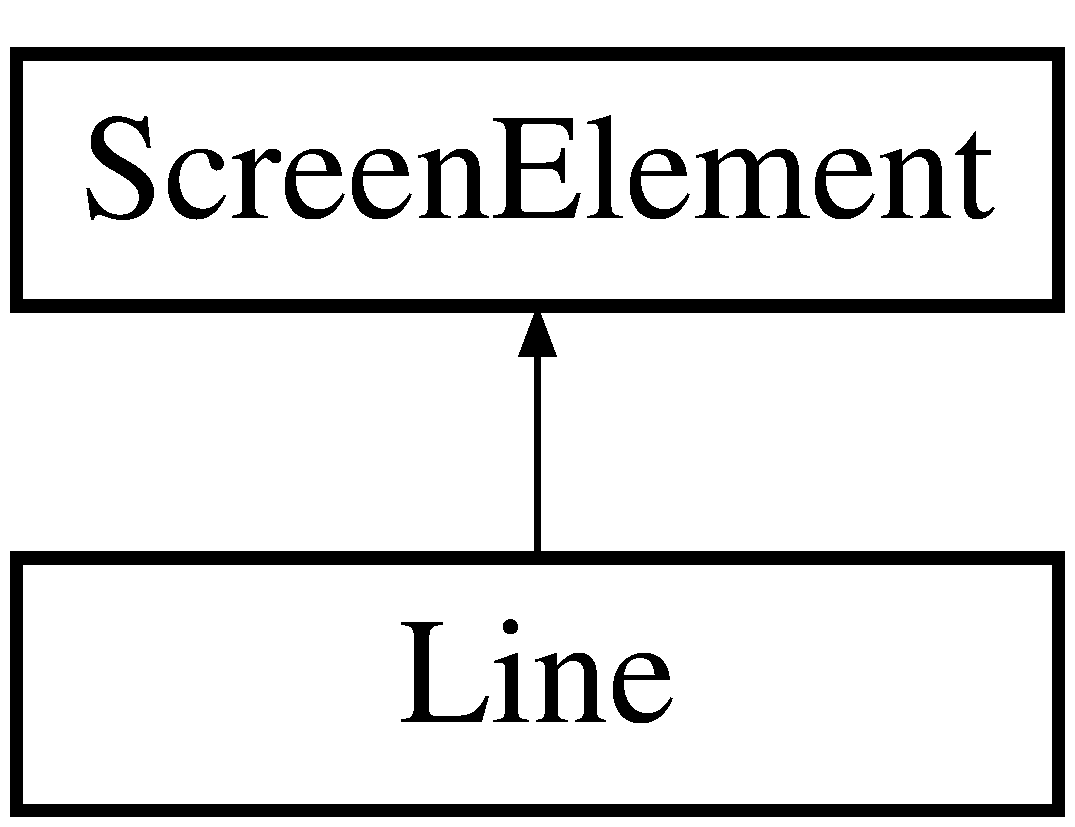
\includegraphics[height=2cm]{classLine}
\end{center}
\end{figure}
\subsection*{Public Member Functions}
\begin{DoxyCompactItemize}
\item 
\hyperlink{classLine_a1012aa02dc32f538f8a677748bd5d328}{Line} (int row1=0, int column1=0, int row2=0, int column2=0, char ch= ' ')
\item 
virtual void \hyperlink{classLine_a0f119b83f7c23a1bf27b6d34f93b63f2}{draw} (\hyperlink{classScreen}{Screen} \&screen)
\begin{DoxyCompactList}\small\item\em draws the line on the given \hyperlink{classScreen}{Screen} \item\end{DoxyCompactList}\item 
virtual void \hyperlink{classLine_a8ca52eabbd2ede5f52cf6c220a4c2f2c}{read} (istream \&is)
\end{DoxyCompactItemize}
\subsection*{Protected Attributes}
\begin{DoxyCompactItemize}
\item 
\hypertarget{classLine_a51f23ff1468a17bb6cfd3b5542bbc016}{
int \hyperlink{classLine_a51f23ff1468a17bb6cfd3b5542bbc016}{m\_\-row1}}
\label{classLine_a51f23ff1468a17bb6cfd3b5542bbc016}

\begin{DoxyCompactList}\small\item\em the row of the first end point \item\end{DoxyCompactList}\item 
\hypertarget{classLine_aac38f7fd7ce511d459918defad228954}{
int \hyperlink{classLine_aac38f7fd7ce511d459918defad228954}{m\_\-col1}}
\label{classLine_aac38f7fd7ce511d459918defad228954}

\begin{DoxyCompactList}\small\item\em the column of the first end point \item\end{DoxyCompactList}\item 
\hypertarget{classLine_a1bf05211608ec421379dd011f7ffff8e}{
int \hyperlink{classLine_a1bf05211608ec421379dd011f7ffff8e}{m\_\-row2}}
\label{classLine_a1bf05211608ec421379dd011f7ffff8e}

\begin{DoxyCompactList}\small\item\em the row of the other end point \item\end{DoxyCompactList}\item 
\hypertarget{classLine_a653ef8926892973fd8e5fdc743f4f5f8}{
int \hyperlink{classLine_a653ef8926892973fd8e5fdc743f4f5f8}{m\_\-col2}}
\label{classLine_a653ef8926892973fd8e5fdc743f4f5f8}

\begin{DoxyCompactList}\small\item\em the column of the other end point \item\end{DoxyCompactList}\item 
\hypertarget{classLine_a57f00e058f608b8c858585fff50d129f}{
char \hyperlink{classLine_a57f00e058f608b8c858585fff50d129f}{m\_\-ch}}
\label{classLine_a57f00e058f608b8c858585fff50d129f}

\begin{DoxyCompactList}\small\item\em the drawing character \item\end{DoxyCompactList}\end{DoxyCompactItemize}


\subsection{Detailed Description}
The \hyperlink{classLine}{Line} class is an abstraction of a vertical or horizontal line that can be drawn on a \hyperlink{classScreen}{Screen}. It is specified internally by two end points, as well as a character to draw the line with. It provides functions to draw itself on a \hyperlink{classScreen}{Screen} as well as reading a description of itself from an input stream. 

\subsection{Constructor \& Destructor Documentation}
\hypertarget{classLine_a1012aa02dc32f538f8a677748bd5d328}{
\index{Line@{Line}!Line@{Line}}
\index{Line@{Line}!Line@{Line}}
\subsubsection[{Line}]{\setlength{\rightskip}{0pt plus 5cm}Line::Line (int {\em row1} = {\ttfamily 0}, \/  int {\em column1} = {\ttfamily 0}, \/  int {\em row2} = {\ttfamily 0}, \/  int {\em column2} = {\ttfamily 0}, \/  char {\em ch} = {\ttfamily '~'})}}
\label{classLine_a1012aa02dc32f538f8a677748bd5d328}
constructs a line


\begin{DoxyParams}{Parameters}
\item[\mbox{$\leftarrow$} {\em row1}]the row of the first end point \item[\mbox{$\leftarrow$} {\em column1}]the column of the first end point \item[\mbox{$\leftarrow$} {\em row2}]the row of the second end point \item[\mbox{$\leftarrow$} {\em column2}]the column of the second end point \item[\mbox{$\leftarrow$} {\em ch}]the drawing character \end{DoxyParams}


\subsection{Member Function Documentation}
\hypertarget{classLine_a0f119b83f7c23a1bf27b6d34f93b63f2}{
\index{Line@{Line}!draw@{draw}}
\index{draw@{draw}!Line@{Line}}
\subsubsection[{draw}]{\setlength{\rightskip}{0pt plus 5cm}virtual void Line::draw ({\bf Screen} \& {\em screen})\hspace{0.3cm}{\ttfamily  \mbox{[}virtual\mbox{]}}}}
\label{classLine_a0f119b83f7c23a1bf27b6d34f93b63f2}


draws the line on the given \hyperlink{classScreen}{Screen} 
\begin{DoxyParams}{Parameters}
\item[\mbox{$\leftrightarrow$} {\em screen}]the screen to draw in \end{DoxyParams}


Implements \hyperlink{classScreenElement_a1bf719edc836cc6ceaa84014c7342028}{ScreenElement}.\hypertarget{classLine_a8ca52eabbd2ede5f52cf6c220a4c2f2c}{
\index{Line@{Line}!read@{read}}
\index{read@{read}!Line@{Line}}
\subsubsection[{read}]{\setlength{\rightskip}{0pt plus 5cm}virtual void Line::read (istream \& {\em is})\hspace{0.3cm}{\ttfamily  \mbox{[}virtual\mbox{]}}}}
\label{classLine_a8ca52eabbd2ede5f52cf6c220a4c2f2c}
reads a description of the line from input stream. The row and columns of the two end points, as well as the drawing character are specified on one line of input separated by spaces. 
\begin{DoxyExceptions}{Exceptions}
\item[{\em \hyperlink{classinput__format__error}{input\_\-format\_\-error}}]\end{DoxyExceptions}

\begin{DoxyParams}{Parameters}
\item[\mbox{$\leftrightarrow$} {\em is}]the input stream to read from \end{DoxyParams}


Implements \hyperlink{classScreenElement_ae5c8356d0faace202bb3ee620433677e}{ScreenElement}.

The documentation for this class was generated from the following files:\begin{DoxyCompactItemize}
\item 
Line.h\item 
Line.cc\end{DoxyCompactItemize}

\hypertarget{classScreen}{
\section{Screen Class Reference}
\label{classScreen}\index{Screen@{Screen}}
}


{\ttfamily \#include $<$Screen.h$>$}\subsection*{Public Member Functions}
\begin{DoxyCompactItemize}
\item 
\hyperlink{classScreen_a44fc6e533a84e710467128a95f20462c}{Screen} (int height=24, int width=80)
\begin{DoxyCompactList}\small\item\em constructs a \hyperlink{classScreen}{Screen} object from the given dimensions \item\end{DoxyCompactList}\item 
int \hyperlink{classScreen_a2d1cf1b84a49135a33aac9d7dc41af3a}{getRows} () const 
\begin{DoxyCompactList}\small\item\em returns the number of rows in the array \item\end{DoxyCompactList}\item 
int \hyperlink{classScreen_ad910656f46d9b22295fb030b5e2aec3d}{getColumns} () const 
\begin{DoxyCompactList}\small\item\em returns the number of columns in the array \item\end{DoxyCompactList}\item 
\hypertarget{classScreen_a35e74266b2a04e37b354ceff7a5f1031}{
void \hyperlink{classScreen_a35e74266b2a04e37b354ceff7a5f1031}{clear} ()}
\label{classScreen_a35e74266b2a04e37b354ceff7a5f1031}

\begin{DoxyCompactList}\small\item\em resets the entire array to spaces \item\end{DoxyCompactList}\item 
void \hyperlink{classScreen_ae19cdc0fab2d48c6bc947a78bb77b50a}{set} (int row, int col, char ch)
\end{DoxyCompactItemize}
\subsection*{Friends}
\begin{DoxyCompactItemize}
\item 
ostream \& \hyperlink{classScreen_aa0d87c1b28233bc47310fb992a0a648e}{operator$<$$<$} (ostream \&os, const \hyperlink{classScreen}{Screen} \&screen)
\begin{DoxyCompactList}\small\item\em output the given \hyperlink{classScreen}{Screen} object to the output stream \item\end{DoxyCompactList}\end{DoxyCompactItemize}


\subsection{Detailed Description}
The \hyperlink{classScreen}{Screen} class is an abstraction of a 2D character array. The coordinates of each location is specified by the row and column. Rows are numbered from 0 from the top, and columns are numbered from 0 from the left. 

\subsection{Constructor \& Destructor Documentation}
\hypertarget{classScreen_a44fc6e533a84e710467128a95f20462c}{
\index{Screen@{Screen}!Screen@{Screen}}
\index{Screen@{Screen}!Screen@{Screen}}
\subsubsection[{Screen}]{\setlength{\rightskip}{0pt plus 5cm}Screen::Screen (int {\em height} = {\ttfamily 24}, \/  int {\em width} = {\ttfamily 80})}}
\label{classScreen_a44fc6e533a84e710467128a95f20462c}


constructs a \hyperlink{classScreen}{Screen} object from the given dimensions 
\begin{DoxyParams}{Parameters}
\item[\mbox{$\leftarrow$} {\em height}]the height of the array, default to 24 \item[\mbox{$\leftarrow$} {\em width}]the width of the array, default to 80 \end{DoxyParams}


\subsection{Member Function Documentation}
\hypertarget{classScreen_ad910656f46d9b22295fb030b5e2aec3d}{
\index{Screen@{Screen}!getColumns@{getColumns}}
\index{getColumns@{getColumns}!Screen@{Screen}}
\subsubsection[{getColumns}]{\setlength{\rightskip}{0pt plus 5cm}int Screen::getColumns () const\hspace{0.3cm}{\ttfamily  \mbox{[}inline\mbox{]}}}}
\label{classScreen_ad910656f46d9b22295fb030b5e2aec3d}


returns the number of columns in the array \begin{DoxyReturn}{Returns}
the number of columns in the array 
\end{DoxyReturn}
\hypertarget{classScreen_a2d1cf1b84a49135a33aac9d7dc41af3a}{
\index{Screen@{Screen}!getRows@{getRows}}
\index{getRows@{getRows}!Screen@{Screen}}
\subsubsection[{getRows}]{\setlength{\rightskip}{0pt plus 5cm}int Screen::getRows () const\hspace{0.3cm}{\ttfamily  \mbox{[}inline\mbox{]}}}}
\label{classScreen_a2d1cf1b84a49135a33aac9d7dc41af3a}


returns the number of rows in the array \begin{DoxyReturn}{Returns}
the number of rows in the array 
\end{DoxyReturn}
\hypertarget{classScreen_ae19cdc0fab2d48c6bc947a78bb77b50a}{
\index{Screen@{Screen}!set@{set}}
\index{set@{set}!Screen@{Screen}}
\subsubsection[{set}]{\setlength{\rightskip}{0pt plus 5cm}void Screen::set (int {\em row}, \/  int {\em col}, \/  char {\em ch})}}
\label{classScreen_ae19cdc0fab2d48c6bc947a78bb77b50a}
sets the character at the given location to the given character. The request is ignored if the location is invalid. 
\begin{DoxyExceptions}{Exceptions}
\item[{\em \hyperlink{classinvalid__coordinates__error}{invalid\_\-coordinates\_\-error}}]\end{DoxyExceptions}

\begin{DoxyParams}{Parameters}
\item[\mbox{$\leftarrow$} {\em row}]row of the location \item[\mbox{$\leftarrow$} {\em col}]column of the location \item[\mbox{$\leftarrow$} {\em ch}]the character to put into the location \end{DoxyParams}


\subsection{Friends And Related Function Documentation}
\hypertarget{classScreen_aa0d87c1b28233bc47310fb992a0a648e}{
\index{Screen@{Screen}!operator$<$$<$@{operator$<$$<$}}
\index{operator$<$$<$@{operator$<$$<$}!Screen@{Screen}}
\subsubsection[{operator$<$$<$}]{\setlength{\rightskip}{0pt plus 5cm}ostream\& operator$<$$<$ (ostream \& {\em os}, \/  const {\bf Screen} \& {\em screen})\hspace{0.3cm}{\ttfamily  \mbox{[}friend\mbox{]}}}}
\label{classScreen_aa0d87c1b28233bc47310fb992a0a648e}


output the given \hyperlink{classScreen}{Screen} object to the output stream 
\begin{DoxyParams}{Parameters}
\item[\mbox{$\leftarrow$} {\em os}]output stream \item[\mbox{$\leftarrow$} {\em screen}]the \hyperlink{classScreen}{Screen} object \end{DoxyParams}
\begin{DoxyReturn}{Returns}
the output stream 
\end{DoxyReturn}


The documentation for this class was generated from the following files:\begin{DoxyCompactItemize}
\item 
Screen.h\item 
Screen.cc\end{DoxyCompactItemize}

\hypertarget{classScreenElement}{
\section{ScreenElement Class Reference}
\label{classScreenElement}\index{ScreenElement@{ScreenElement}}
}


{\ttfamily \#include $<$ScreenElement.h$>$}Inheritance diagram for ScreenElement::\begin{figure}[H]
\begin{center}
\leavevmode
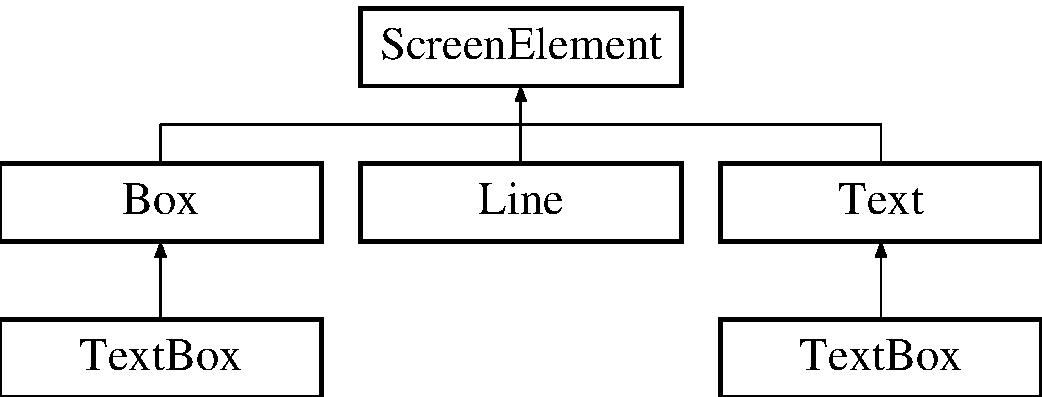
\includegraphics[height=3cm]{classScreenElement}
\end{center}
\end{figure}
\subsection*{Public Member Functions}
\begin{DoxyCompactItemize}
\item 
\hypertarget{classScreenElement_ae88aa724a30f2aa3b24576a0b8b1ed43}{
virtual \hyperlink{classScreenElement_ae88aa724a30f2aa3b24576a0b8b1ed43}{$\sim$ScreenElement} ()}
\label{classScreenElement_ae88aa724a30f2aa3b24576a0b8b1ed43}

\begin{DoxyCompactList}\small\item\em destroys the object \item\end{DoxyCompactList}\item 
virtual void \hyperlink{classScreenElement_a1bf719edc836cc6ceaa84014c7342028}{draw} (\hyperlink{classScreen}{Screen} \&screen)=0
\begin{DoxyCompactList}\small\item\em draws the element on the given \hyperlink{classScreen}{Screen} \item\end{DoxyCompactList}\item 
virtual void \hyperlink{classScreenElement_ae5c8356d0faace202bb3ee620433677e}{read} (istream \&is)=0
\begin{DoxyCompactList}\small\item\em reads a description of the element from input stream \item\end{DoxyCompactList}\end{DoxyCompactItemize}


\subsection{Detailed Description}
The \hyperlink{classScreenElement}{ScreenElement} class is an abstraction of any element that can appear on a \hyperlink{classScreen}{Screen}. It provides functions to draw itself on a \hyperlink{classScreen}{Screen} as well as reading a description of itself from an input stream. 

\subsection{Member Function Documentation}
\hypertarget{classScreenElement_a1bf719edc836cc6ceaa84014c7342028}{
\index{ScreenElement@{ScreenElement}!draw@{draw}}
\index{draw@{draw}!ScreenElement@{ScreenElement}}
\subsubsection[{draw}]{\setlength{\rightskip}{0pt plus 5cm}virtual void ScreenElement::draw ({\bf Screen} \& {\em screen})\hspace{0.3cm}{\ttfamily  \mbox{[}pure virtual\mbox{]}}}}
\label{classScreenElement_a1bf719edc836cc6ceaa84014c7342028}


draws the element on the given \hyperlink{classScreen}{Screen} 
\begin{DoxyParams}{Parameters}
\item[\mbox{$\leftrightarrow$} {\em screen}]the screen to draw in \end{DoxyParams}


Implemented in \hyperlink{classBox_a5c6c1c650b13f2978e3b559bb5af15d2}{Box}, \hyperlink{classLine_a0f119b83f7c23a1bf27b6d34f93b63f2}{Line}, \hyperlink{classText_a5fedb2f5b4c40b9cd8965d58716b73f8}{Text}, and \hyperlink{classTextBox_ae28a00e6cd50d5432c02b579b0fb32ed}{TextBox}.\hypertarget{classScreenElement_ae5c8356d0faace202bb3ee620433677e}{
\index{ScreenElement@{ScreenElement}!read@{read}}
\index{read@{read}!ScreenElement@{ScreenElement}}
\subsubsection[{read}]{\setlength{\rightskip}{0pt plus 5cm}virtual void ScreenElement::read (istream \& {\em is})\hspace{0.3cm}{\ttfamily  \mbox{[}pure virtual\mbox{]}}}}
\label{classScreenElement_ae5c8356d0faace202bb3ee620433677e}


reads a description of the element from input stream 
\begin{DoxyParams}{Parameters}
\item[\mbox{$\leftrightarrow$} {\em is}]the input stream to read from \end{DoxyParams}


Implemented in \hyperlink{classBox_ac0ea633a10bf980901766b7aaefdb912}{Box}, \hyperlink{classLine_a8ca52eabbd2ede5f52cf6c220a4c2f2c}{Line}, \hyperlink{classText_af326f364609eb7e286ad778accb29db3}{Text}, and \hyperlink{classTextBox_a3265df3298f92813667d1c70479f7f5c}{TextBox}.

The documentation for this class was generated from the following file:\begin{DoxyCompactItemize}
\item 
ScreenElement.h\end{DoxyCompactItemize}

\hypertarget{classText}{
\section{Text Class Reference}
\label{classText}\index{Text@{Text}}
}


{\ttfamily \#include $<$Text.h$>$}Inheritance diagram for Text::\begin{figure}[H]
\begin{center}
\leavevmode
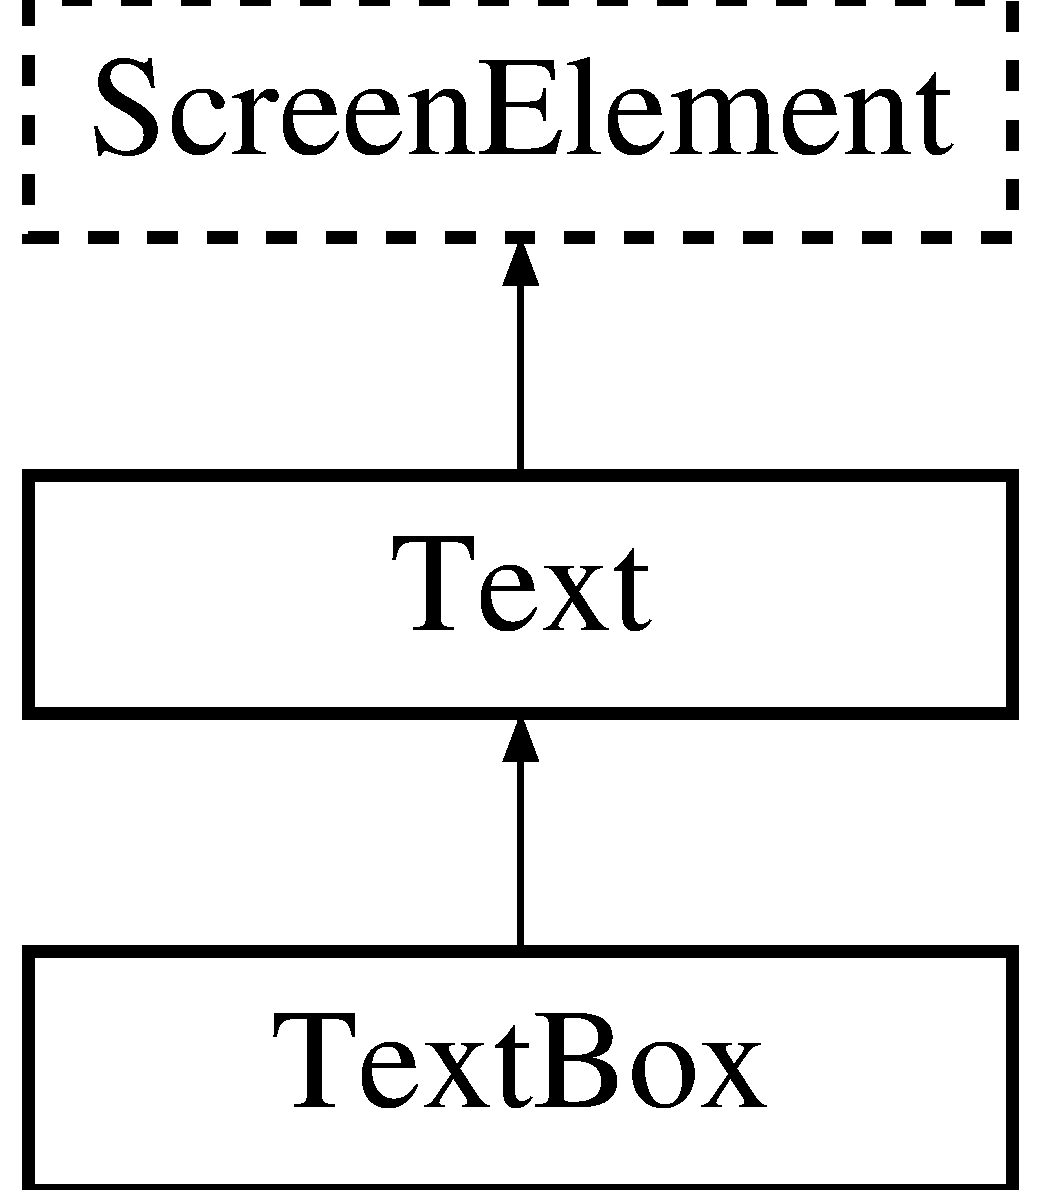
\includegraphics[height=3cm]{classText}
\end{center}
\end{figure}
\subsection*{Public Member Functions}
\begin{DoxyCompactItemize}
\item 
\hyperlink{classText_a1c798d677585c623ce9cd6b9d874cafe}{Text} (int row=0, int column=0, const string \&str=\char`\"{}\char`\"{})
\item 
virtual void \hyperlink{classText_a5fedb2f5b4c40b9cd8965d58716b73f8}{draw} (\hyperlink{classScreen}{Screen} \&screen)
\begin{DoxyCompactList}\small\item\em draws the \hyperlink{classText}{Text} on the given \hyperlink{classScreen}{Screen} \item\end{DoxyCompactList}\item 
virtual void \hyperlink{classText_af326f364609eb7e286ad778accb29db3}{read} (istream \&is)
\end{DoxyCompactItemize}
\subsection*{Protected Attributes}
\begin{DoxyCompactItemize}
\item 
\hypertarget{classText_a32b3be97b9aabe0a490787c7120b371d}{
int \hyperlink{classText_a32b3be97b9aabe0a490787c7120b371d}{m\_\-row}}
\label{classText_a32b3be97b9aabe0a490787c7120b371d}

\begin{DoxyCompactList}\small\item\em The row of the first character. \item\end{DoxyCompactList}\item 
\hypertarget{classText_a09523ee86a807344c5e41db7ccc6ddf2}{
int \hyperlink{classText_a09523ee86a807344c5e41db7ccc6ddf2}{m\_\-col}}
\label{classText_a09523ee86a807344c5e41db7ccc6ddf2}

\begin{DoxyCompactList}\small\item\em The column of the first character. \item\end{DoxyCompactList}\item 
\hypertarget{classText_aead900be403332c4d7c9388e6a1be316}{
string \hyperlink{classText_aead900be403332c4d7c9388e6a1be316}{m\_\-text}}
\label{classText_aead900be403332c4d7c9388e6a1be316}

\begin{DoxyCompactList}\small\item\em The text string. \item\end{DoxyCompactList}\end{DoxyCompactItemize}


\subsection{Detailed Description}
The \hyperlink{classText}{Text} class is an abstraction of a text string that can be drawn on a \hyperlink{classScreen}{Screen}. It is specified internally by the location of the first character and the string itself. It provides functions to draw itself on a \hyperlink{classScreen}{Screen} as well as reading a description of itself from an input stream. 

\subsection{Constructor \& Destructor Documentation}
\hypertarget{classText_a1c798d677585c623ce9cd6b9d874cafe}{
\index{Text@{Text}!Text@{Text}}
\index{Text@{Text}!Text@{Text}}
\subsubsection[{Text}]{\setlength{\rightskip}{0pt plus 5cm}Text::Text (int {\em row} = {\ttfamily 0}, \/  int {\em column} = {\ttfamily 0}, \/  const string \& {\em str} = {\ttfamily \char`\"{}\char`\"{}})}}
\label{classText_a1c798d677585c623ce9cd6b9d874cafe}
constructs a text object


\begin{DoxyParams}{Parameters}
\item[\mbox{$\leftarrow$} {\em row}]the row of the first character \item[\mbox{$\leftarrow$} {\em column}]the column of the first character \item[\mbox{$\leftarrow$} {\em str}]the string \end{DoxyParams}


\subsection{Member Function Documentation}
\hypertarget{classText_a5fedb2f5b4c40b9cd8965d58716b73f8}{
\index{Text@{Text}!draw@{draw}}
\index{draw@{draw}!Text@{Text}}
\subsubsection[{draw}]{\setlength{\rightskip}{0pt plus 5cm}virtual void Text::draw ({\bf Screen} \& {\em screen})\hspace{0.3cm}{\ttfamily  \mbox{[}virtual\mbox{]}}}}
\label{classText_a5fedb2f5b4c40b9cd8965d58716b73f8}


draws the \hyperlink{classText}{Text} on the given \hyperlink{classScreen}{Screen} 
\begin{DoxyParams}{Parameters}
\item[\mbox{$\leftrightarrow$} {\em screen}]the screen to draw in \end{DoxyParams}


Implements \hyperlink{classScreenElement_a1bf719edc836cc6ceaa84014c7342028}{ScreenElement}.

Reimplemented in \hyperlink{classTextBox_ae28a00e6cd50d5432c02b579b0fb32ed}{TextBox}.\hypertarget{classText_af326f364609eb7e286ad778accb29db3}{
\index{Text@{Text}!read@{read}}
\index{read@{read}!Text@{Text}}
\subsubsection[{read}]{\setlength{\rightskip}{0pt plus 5cm}virtual void Text::read (istream \& {\em is})\hspace{0.3cm}{\ttfamily  \mbox{[}virtual\mbox{]}}}}
\label{classText_af326f364609eb7e286ad778accb29db3}
reads a description of the \hyperlink{classText}{Text} from input stream. The row and column of the first character, as well as the text string are specified on one line of input separated by spaces. 
\begin{DoxyExceptions}{Exceptions}
\item[{\em \hyperlink{classinput__format__error}{input\_\-format\_\-error}}]\end{DoxyExceptions}

\begin{DoxyParams}{Parameters}
\item[\mbox{$\leftrightarrow$} {\em is}]the input stream to read from \end{DoxyParams}


Implements \hyperlink{classScreenElement_ae5c8356d0faace202bb3ee620433677e}{ScreenElement}.

Reimplemented in \hyperlink{classTextBox_a3265df3298f92813667d1c70479f7f5c}{TextBox}.

The documentation for this class was generated from the following files:\begin{DoxyCompactItemize}
\item 
Text.h\item 
Text.cc\end{DoxyCompactItemize}

\hypertarget{classTextBox}{
\section{TextBox Class Reference}
\label{classTextBox}\index{TextBox@{TextBox}}
}


{\ttfamily \#include $<$TextBox.h$>$}Inheritance diagram for TextBox::\begin{figure}[H]
\begin{center}
\leavevmode
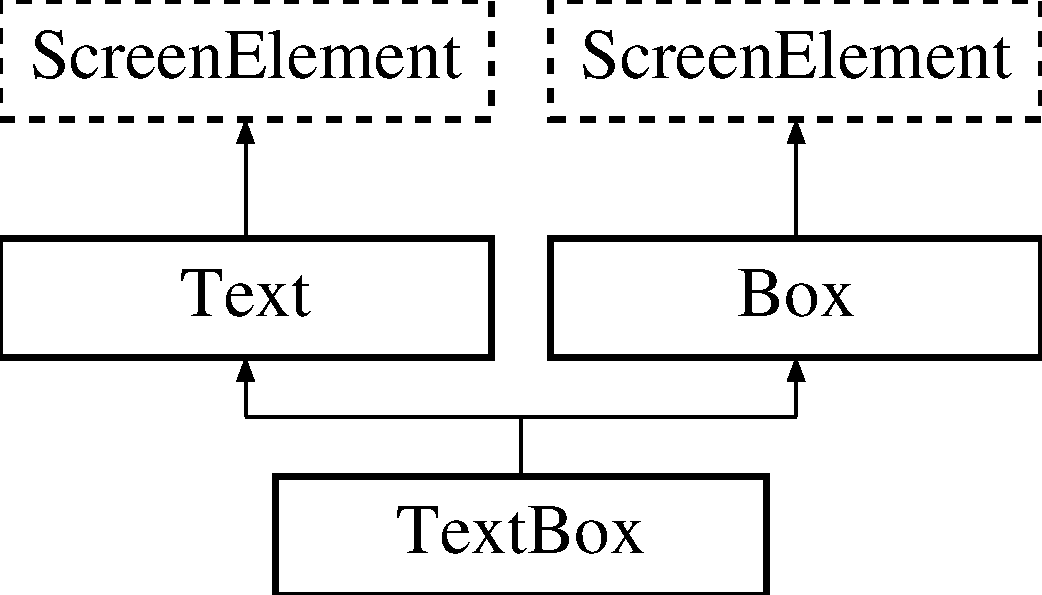
\includegraphics[height=3cm]{classTextBox}
\end{center}
\end{figure}
\subsection*{Public Member Functions}
\begin{DoxyCompactItemize}
\item 
\hyperlink{classTextBox_ac0d2d825a2ca3f37f8d417c437032d71}{TextBox} (int row=0, int column=0, char ch= ' ', const string \&str=\char`\"{}\char`\"{})
\item 
virtual void \hyperlink{classTextBox_ae28a00e6cd50d5432c02b579b0fb32ed}{draw} (\hyperlink{classScreen}{Screen} \&screen)
\begin{DoxyCompactList}\small\item\em draws the \hyperlink{classTextBox}{TextBox} on the given \hyperlink{classScreen}{Screen} \item\end{DoxyCompactList}\item 
virtual void \hyperlink{classTextBox_a3265df3298f92813667d1c70479f7f5c}{read} (istream \&is)
\end{DoxyCompactItemize}


\subsection{Detailed Description}
The \hyperlink{classTextBox}{TextBox} class is an abstraction of a rectangular box containing a text string that can be drawn on a \hyperlink{classScreen}{Screen}. It provides functions to draw itself on a \hyperlink{classScreen}{Screen} as well as reading a description of itself from an input stream. 

\subsection{Constructor \& Destructor Documentation}
\hypertarget{classTextBox_ac0d2d825a2ca3f37f8d417c437032d71}{
\index{TextBox@{TextBox}!TextBox@{TextBox}}
\index{TextBox@{TextBox}!TextBox@{TextBox}}
\subsubsection[{TextBox}]{\setlength{\rightskip}{0pt plus 5cm}TextBox::TextBox (int {\em row} = {\ttfamily 0}, \/  int {\em column} = {\ttfamily 0}, \/  char {\em ch} = {\ttfamily '~'}, \/  const string \& {\em str} = {\ttfamily \char`\"{}\char`\"{}})}}
\label{classTextBox_ac0d2d825a2ca3f37f8d417c437032d71}
constructs a \hyperlink{classTextBox}{TextBox}


\begin{DoxyParams}{Parameters}
\item[\mbox{$\leftarrow$} {\em row}]the row of the first character \item[\mbox{$\leftarrow$} {\em column}]the column of the first character \item[\mbox{$\leftarrow$} {\em ch}]the drawing character for the box \item[\mbox{$\leftarrow$} {\em str}]the string \end{DoxyParams}


\subsection{Member Function Documentation}
\hypertarget{classTextBox_ae28a00e6cd50d5432c02b579b0fb32ed}{
\index{TextBox@{TextBox}!draw@{draw}}
\index{draw@{draw}!TextBox@{TextBox}}
\subsubsection[{draw}]{\setlength{\rightskip}{0pt plus 5cm}virtual void TextBox::draw ({\bf Screen} \& {\em screen})\hspace{0.3cm}{\ttfamily  \mbox{[}virtual\mbox{]}}}}
\label{classTextBox_ae28a00e6cd50d5432c02b579b0fb32ed}


draws the \hyperlink{classTextBox}{TextBox} on the given \hyperlink{classScreen}{Screen} 
\begin{DoxyParams}{Parameters}
\item[\mbox{$\leftrightarrow$} {\em screen}]the screen to draw in \end{DoxyParams}


Reimplemented from \hyperlink{classBox_a5c6c1c650b13f2978e3b559bb5af15d2}{Box}.\hypertarget{classTextBox_a3265df3298f92813667d1c70479f7f5c}{
\index{TextBox@{TextBox}!read@{read}}
\index{read@{read}!TextBox@{TextBox}}
\subsubsection[{read}]{\setlength{\rightskip}{0pt plus 5cm}virtual void TextBox::read (istream \& {\em is})\hspace{0.3cm}{\ttfamily  \mbox{[}virtual\mbox{]}}}}
\label{classTextBox_a3265df3298f92813667d1c70479f7f5c}
reads a description of the \hyperlink{classTextBox}{TextBox} from input stream. The row and column of the first character, the drawing character of the box, as well as the string are specified on one line of input separated by spaces. 
\begin{DoxyExceptions}{Exceptions}
\item[{\em \hyperlink{classinput__format__error}{input\_\-format\_\-error}}]\end{DoxyExceptions}

\begin{DoxyParams}{Parameters}
\item[\mbox{$\leftrightarrow$} {\em is}]the input stream to read from \end{DoxyParams}


Reimplemented from \hyperlink{classBox_ac0ea633a10bf980901766b7aaefdb912}{Box}.

The documentation for this class was generated from the following files:\begin{DoxyCompactItemize}
\item 
TextBox.h\item 
TextBox.cc\end{DoxyCompactItemize}

\printindex
\end{document}
